\chapter{Vers les bases de données graphe}
\label{ch:graph-db}
Avec le développement rapide et continu de l'Internet et le cloud
computing, divers types d'applications ont émergés, ce qui augmente
l'mportance accrue de la technologie de base de données, notamment
dans les aspects suivants \cite{han2011survey}:

\begin{itemize}
\item Haute concurrente de lecture et d'écriture avec une faible
  latence.
\item Stockage et la gestion d'une grande masse de données \emph{(Big
    Data)}.
\item Haute scalabilité (évolutivité) et disponibilité.
\end{itemize}

Bien que les bases de données relationnelles ont occupé une grande
position dans le domaine de stockage de données, le modèle relationnel
commençait à montrer ses limites en faisant face au-dessus exigences
\cite{han2011survey}:

\begin{itemize}
\item Lente lecture et l'écriture.
\item Capacité limitée.
\item Difficulté d'expansion et scalabilité.
\end{itemize}

Afin de faire face aux limitations ci-dessus, une variété de nouveaux
types de bases de données ont été apparus qui s'affranchissent du
modèle relationnel pour miser sur le partitionnement horizontal et le
relâchement des contraintes d'intégrité, ce modèle émergent est appelé
le modèle \acrshort{nosql}.

Dans ce chapitre, nous exposons les différentes approches et
plateformes du stockage \textsc{NoSQL} les plus connues dans
l'industrie tout en mettant l'accent sur les bases de données graphes
(et \emph{Neo4j} particulièrement). Nous commençons d'abord par
présenter les quatre catégories majeurs des systèmes
\textsc{NoSQL}. Ensuite, nous focalisons sur les \acrshort{SGBD}
orientés graphes, leurs différents modèles et implémentations ainsi
que les langages de requêtes les plus adoptés pour les interroger.

\section{L'environnement NoSQL}
\label{sec:nosql}
% TODO: make a real definition
\acrshort{nosql} désigne une catégorie de systèmes de gestion de base
de données (\acrshort{SGBD}) qui n'est plus fondée sur l'architecture
classique des bases relationnelles. L'unité logique n'y est plus la
table, et les données ne sont en général pas manipulées avec
\textsc{SQL}. À l'origine, servant à manipuler des bases de données
géantes pour des sites web de très grande audience tels que Google
Amazon, Facebook et eBay. D'aprés Martin fowler \textit{et al.}
\cite{sadalage2012nosql}, Les caractéristiques communes des bases de
données \acrshort{nosql} sont:

\begin{itemize}
\item Ne sont pas fondées sur de le modèle relationnel classique.
\item Optimisées pour les environments distribués.
\item Généralement sous des licences \emph{Open Source}.
\item Construites pour les applications Web modernes avec une grande
  masse de données.
\item \emph{Schemaless} (il n'existe plus d'intégrité référentielle ou
  schémas prédéfini).
\end{itemize}

  \subsection{Catégories des bases de données NoSQL}
  \label{sec:cat-nosql}
  Il existe dans la mouvance \acrshort{nosql} une diversité importante
  d'approches. que nous classons en quatre grandes catégories : dépots
  clés/valeurs, bases orientées documents, orientées colonnes, et
  bases orientées graphes.

  \begin{itemize}
  \item [Dépots clés/valeurs]: Le principe des bases
    \textit{clé/valeur} est de stocker les données sous une forme
    simple: une \emph{clé } (chaîne de caractères) associé à une
    \emph{valeur} d'une forme libre (chaîne de caractère, nombre ou
    bien un objet sérialisé), cette clé est utilisée pout toutes les
    opérations à effectuer sur les données telles que l'insertion, la
    mise à jour et la supression. Bien que la structure est plus
    simple, la vitesse d'interrogation est extrêmement supérieur à la
    base de données relationnelles favorisant la scalabilité
    (\emph{scalability}) plus que la cohérence, on les retrouve très
    souvent comme système de stockage de cache ou de sessions
    distribuées, notamment là où l'intégrité relationnelle des données
    est non significative. Les solutions les plus connues, telle que
    \emph{Redis}, \emph{Riak} et \emph{Voldemort} sont principalement
    influencés par le project \emph{Dynamo} d'Amazon
    \cite{decandia2007dynamo}.
    \newpage

  \item [Orientées documents]: Cette famille de base de données est
    une évolution de la base de données \textit{clé/valeur} destinée
    aux applications qui gèrent des documents (généralement du format
    \textsc{JSON} ou \textsc{XML}) où chaque clé n'est plus associée à
    une valeur sous forme de bloc binaire mais à un document dont la
    structure reste libre (\textit{scheme-less}). L'avantage est de
    pouvoir récupérer, via une seule clé, un ensemble d’informations
    structurées de manière hiérarchique. ansi que le stockage de
    volumes très importants de données pour lesquelles la modélisation
    relationnelle aurait entraînée une limitation des possibilités de
    partitionnement et de réplication. les deux implémentations les
    plus populaires dans cette catégorie sont \emph{CouchDB} d'Apache
    et \emph{MongoDB}.

  \item [Orientées colonnes]: Une base de données orientée colonnes
    est une base de données qui stocke les données par colonne et non
    par ligne. L'orientation colonne permet d'ajouter des colonnes
    plus facilement aux tables (les lignes n'ont pas besoin d'être
    redimensionnées). Elle permet de plus une compression par colonne,
    efficace lorsque les données de la colonne se ressemblent. Comme
    solutions, on retrouve principalement \emph{HBase},
    \emph{HyperTable} (implémentations Open Source du modèle
    \emph{BigTable} \cite{chang2008bigtable} publié par Google) ainsi
    que \emph{Cassandra} (projet Apache qui respecte l'architecture
    distribuée de \emph{Dynamo} \cite{decandia2007dynamo} d'Amazon et
    le modèle BigTable de Google).

  \item [Orientées graphes]: Ce paradigme est le moins connu de ceux
    de la mouvance \acrshort{nosql}. Ce modèle s'appuie principalement
    sur deux concepts: d'une part l'utilisation d'un moteur de
    stockage pour les objets (qui se présentent sous la forme d'une
    base documentaire, chaque entité de cette base étant nommée
    \emph{nœud}). D'autre part, à ce modèle, vient s'ajouter un
    mécanisme permettant de décrire les relations entre les objets
    (\emph{arcs}). Principalement, ces bases de données sont nettement
    plus efficaces que leur pendant relationnel pour traiter les
    problématiques liées aux réseaux.  En effet, lorsqu'on utilise le
    modèle relationnel, cela nécessite un grand nombre d'opérations
    complexes (souvent, des jointures trop lentes) pour obtenir des
    résultats. Dans cette catégorie on peut citer \emph{Neo4j},
    \emph{OrientDB}, \emph{Titan} et \emph{AllegroGraph} comme les
    implémentations les plus répondus de ce modèle.
  \end{itemize}

  \subsection{Le théorème de CAP }
  \label{sec:cap}

  \acrshort{cap} \cite{brewer2000towards} est l'acronyme de
  \textit{``\textbf{C}onsistency, \textbf{A}vailability and
    \textbf{P}artition Tolerance''}, ou \textit{``Cohérence,
    Disponibilité et Résistance au partitionnement''}. Ce théorème
  explique qu'il est impossible qu'un système distribué satisfasse
  simultanément aux trois contraintes suivantes:

  \begin{itemize}
  \item [Cohérence]: tous les nœuds du système voient exactement les
    mêmes données au même moment.

  \item [Disponibilité]: la perte de nœuds n'empêche pas les survivants
    de continuer à fonctionner correctement.

  \item [Résistance au partitionnement]: aucune panne moins importante
    qu'une coupure totale du réseau ne doit empêcher le système de
    répondre correctement (ou encore : en cas de partitionnement ,
    chacune des partitions doit pouvoir fonctionner de manière
    autonome).
  \end{itemize}

  \begin{figure}[h]
    \centering
    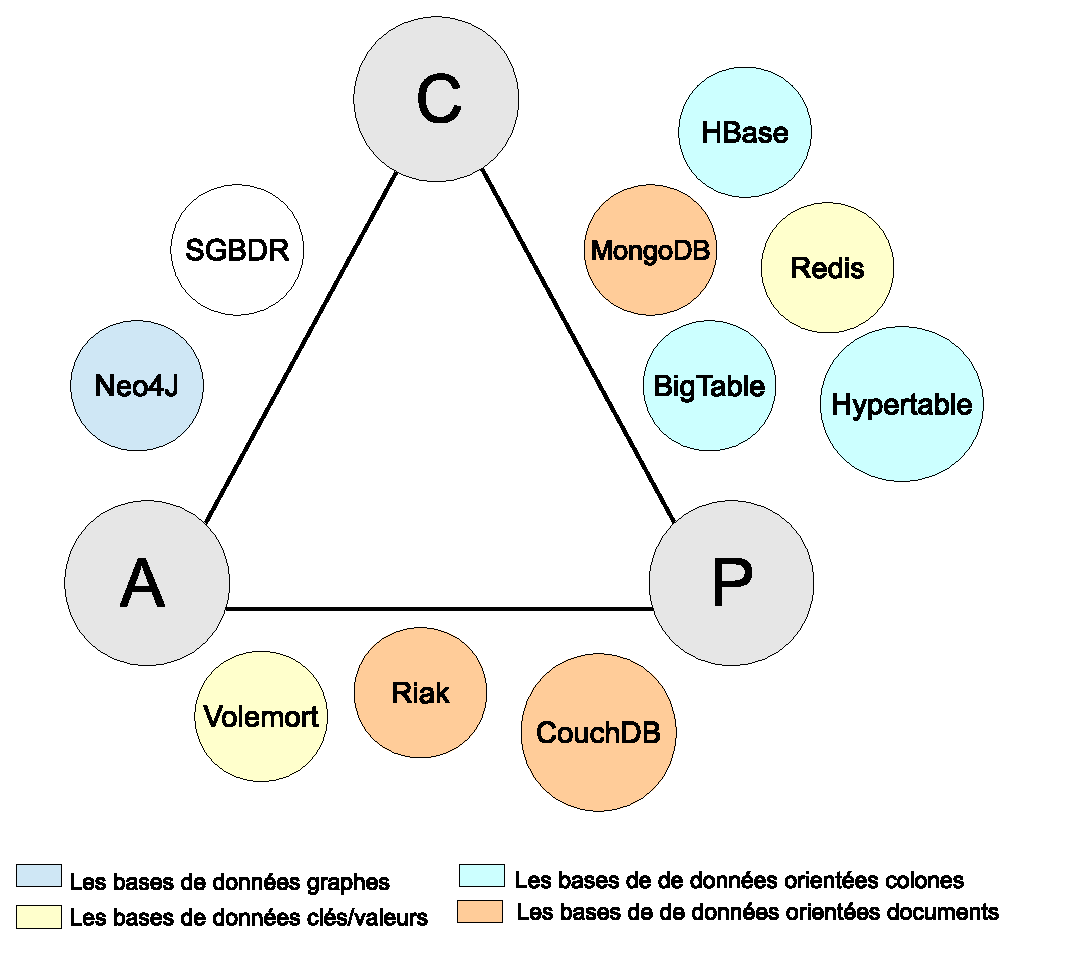
\includegraphics[width=0.96\textwidth]{figs/cap.eps}
    \caption{Le théorème CAP}
    \label{fig:cap}
\end{figure}

%%% Local Variables:
%%% mode: latex
%%% TeX-master: "../main"
%%% End:


  Le théorème de \acrshort{cap} stipule qu'il est impossible d'obtenir
  ces trois propriétés en même temps dans un système distribué et
  qu'il faut donc en choisir deux parmi les trois, Les bases de
  données relationnelles implémentent les propriétés de cohérence et
  de disponibilité (système \emph{CA}). Les bases de données
  \emph{NoSQL} sont généralement des systèmes \emph{CP} (cohérent et
  résistant au partitionnement) ou \emph{AP} (disponible et résistant
  au partitionnement), ce qui illustré dans La figure \ref{fig:cap}
  ci-dessus.



\section{Bases de données orientées graphes}
\label{sec:graph-database-overview}
% TODO: rewrite the intro
\begin{text}
  Un grand nombre de problèmes pratiques dans différentes disciplines
  peuvent être intuitivement représentés sous forme de graphes : des
  nœuds reliés par des arcs (étiqueté ou non).

  Depuis plusieurs décennies, les développeurs ont essayé de stoker
  des ensembles de données connectés, semi-structurées à l'intérieur
  des bases de données relationnelles. Mais alors que les bases de
  données relationnelles ont été initialement conçues pour codifier
  des structures tabulaires. Cependant, les données fortement
  connectées sont traitées de manière très pauvre par les bases de
  données relationnelles. Chaque opération sur une relation dans un
  graphes ou réseau résulte en une opération de jointure dans le
  \acrshort{SGBDR}, implémentée comme une opération ensembliste entre
  l'ensemble des clés primaires de deux tables - une opération lente
  et sans capacité à monter en charge alors que le nombre de t-uples
  de ces tables augmente \cite{robinson2013graph}.

  Les bases de données orientées graphes sont donc conçues pour
  modéliser des réseaux de données fortement connectées et y naviguer
  facilement en bénéficiant de performances extrêmement élevées – un
  atout qui explique leur succès auprès de
  Facebook\footnote{\url{http://www.facebook.com}},
  LinkedIn\footnote{\url{http://www.linkedin.com}} et autres réseaux
  sociaux. Ces derniers sont devenus ces dernières années l'un de cas
  d'utilisation les plus visibles des bases de données graphes.
  LinkedIn parvient ainsi facilement à afficher le degré de séparation
  entre chaque contact, qui n'est finalement que la distance entre les
  nœuds dans le graphes représentant les personnes et leurs relations.
\end{text}

% TODO: relational vs graph database
  \subsection{Techniques de persistance des bases de données graphes}
  \label{sec:persistence-tech}

  \begin{itemize}
  \item [Bases de données graphes au-dessus de d'un stockage SQL]
  \item [Bases de données graphes au-dessus d'un stackages NoSQL]
  \item [Les bases de données graphes natives]
  \end{itemize}

  \subsection{Détails d'implémentation}
  \label{graph-internals}
  \begin{itemize}
  \item [Index-free adjacency]
  \item [Vertex Centric Indices]
  \item [Bitmaps representation of graphs]
  \item [Write Ahead Log]
  \end{itemize}

  \subsection{Comparaison}
  \label{graphdb-comp}

\newpage
\section{Langages d'interrogation des bases de données graphes}
\label{query-languages}

Les langages de requêtes ont toujours été la clé du succès des
systèmes de gestion des bases de données. La prévalence des
\emph{\acrshort{SGBDR}} dans les dernières décennies est étroitement
couplé avec le succès du \emph{SQL}. Des divers langages ont été
définis pour exprimer des requêtes vis-à-vis plusieurs dépôts de
données, par exemple, \emph{XQuery} \cite{boag2002xquery} et
\emph{XPath} \cite{clark1999xml} pour les bases de données
\emph{\acrshort{xml}}, \emph{QQL} \cite{alashqur1989oql} pour les
bases de données orientées objets et \acrshort{sparql}
\cite{prud2008sparql} pour les triplestores (les bases de données
\emph{RDF}). Dans cette section on va présenter les langages de
requêtes les plus utilisée pour l'interrogation des bases de données
graphes.

  % TODO: make a simple graph example
  \subsection{SPARQL}
  \label{sec:sparql}

  \acrshort{sparql} \cite{prud2008sparql} est un langage populaire de
  requêtes pour les données \acrshort{rdf}, il est reconnu comme l'une
  des technologies clés du Web sémantique. Le standard
  \acrshort{sparql} est largement utilisé pour exprimer des
  interrogations à travers diverses sources de données graphes vues
  comme des triplestores \acrshort{rdf}. Il est capable de rechercher
  des motifs de graphe (\emph{graph patterns}) ainsi que leurs
  conjonctions et leurs disjonctions. Les résultats des interrogations
  \textsc{SPARQL} peuvent être des ensembles de résultats ou des
  graphes \acrshort{rdf} qui peuvent être retournés via
  \acrshort{http} dans une variété de formats tels que \acrshort{xml},
  HTML ou \acrshort{json}

  % syntaxe
  % example
  % graph-db support

  {\color{red} \textsc{SPARQL} is supported by some databases such as
    AllegroGraph natively. Other graph databases like Neo4j also
    support \textsc{SPARQL} by applying plugin Linked Data.  }



  \subsection{Gremlin}
  \label{sec:gremlin}
  \emph{Gremlin} \cite{gremlin-wiki} est un langage de domaine
  spécifique (\acrshort{DSL}) de bas niveau pour le parcours des
  graphes attribués, il trouve ses applications dans les domaines de
  la recherche, l'analyse et la manipulation des bases de données
  orientées graphes qui implémentent le modèle \emph{Blueprints}
  \cite{blueprints} de données. \emph{Gremlin} \cite{gremlin-wiki} est
  un projet open source développé et maintenu par \emph{TinkerPop}.

  Le syntaxe \emph{Gremlin} est basée sur \emph{XPath} de manière à
  être capable d'exprimer des descriptions de parcours même profonds
  avec des expressions simples et compactes.

  % example

  La distribution \emph{Gremlin} (maintenu par \emph{TinkerPop}) est
  supporté par la plupart des bases de données graphes via des
  langages \emph{JVM} comme \emph{Java}, \emph{Groovy} et
  \emph{Scala}, parmi ces \acrshort{SGBD} graphes nous trouvons
  \emph{Neo4j}, \emph{Titan} et \emph{OrientDB}.

  \subsection{Cypher}
  \label{sec:cypher}
  \emph{Cypher} \cite{cypher-docs} est un langage des requêtes
  déclaratif pour interagir avec les bases des données graphes
  \emph{Neo4j}, développé et maintenu par \emph{Neo Technology}. Il
  permet d'effectuer des requêtes et mises jour du graphe efficaces
  sans avoir écrire de traversiers (parcours) d'une manière
  procédurale.

  En étant un langage déclaratif, \emph{Cypher} se concentre sur la
  clarté d'exprimer \textit{quoi retrouver dans un graphe et non
    comment le faire}. Ceci est en contraste aux langages impératifs
  comme Java et aux langages script comme \emph{Gremlin}
  \ref{sec:gremlin}, ce qui rend le fait d'optimisation de requêtes un
  détail d'implémentation non exposé aux utilisateurs. \emph{Cypher}
  est inspiré de plusieurs approches et construit sur des pratiques
  établies pour l'interrogation expressif des bases de données. La
  plupart des mots clés comme \verb|WHERE| et \verb|ORDER BY|, et La
  concordance de patterns sont hérités directement des langages
  déclaratifs comme \emph{SQL} et \emph{SPARQL} \ref{sec:sparql} avec
  quelque propriétés inspirés des langages fonctionnels comme
  \emph{Haskell} et \emph{ML}.

  Le langage \emph{Cypher} comporte un nombre de clauses distinctes,
  des clauses pour l'interrogation du graphe comme:
  \begin{itemize}
  \item [\texttt{MATCH}]: Utilisé pour pour décrire Le pattern du graphe
    à correspondre, principalement sur la base de relations entre les
    nœuds du graphe.
  \item [\texttt{WHERE}]: Sert à un critère de filtrage.
  \item [\texttt{RETURN}]: Spécifie ce qu'il faut retourner comme
    résultat finale de requête.
  \end{itemize}

  \emph{Cypher} contient en outre des clauses pour l'écriture, la mise
  à jour et suppression de données, par exemple:

  \begin{itemize}
  \item [\texttt{CREATE}]: Crée des nœuds ou des relations.
  \item [\texttt{SET}]: Affecte des valeurs aux propriétés..
  \item [\texttt{DELETE}]: supprime des noeuds, relations ou propriétés.
  \end{itemize}

  % graph-db support

  % TODO:comparaison

  \section{Conclusion}

  % TODO: Neo4j internals
%%% Local Variables:
%%% mode: latex
%%% TeX-master: "../main"
%%% End:
